\documentclass{article}
\usepackage[a4paper,left=3cm, right=3cm, top=2cm, bottom=2cm]{geometry}
\usepackage{amsmath}
\usepackage{graphicx}
\usepackage{caption}
\usepackage{setspace}
\usepackage{xcolor}
\usepackage{titlesec}
\usepackage{amssymb}
\usepackage{tcolorbox}
\usepackage{wrapfig}
\usepackage{amsthm} % For proofs

% --- 스타일 설정 ---
\graphicspath{{graph/}}
\title{11.1 Sequences}
\date{}
\author{}
\setstretch{1.3} 

% 섹션 제목 스타일 (파란색)
\titleformat{name=\section, numberless}
  {\normalfont\large\bfseries\color{blue}}
  {}
  {0pt}
  {}
% 하위 섹션 제목 스타일 (굵게)
\titleformat{name=\subsection, numberless
}
  {\normalfont\bfseries}
  {}
  {0pt}
  {}
\geometry{a4paper, margin=1in}

% 증명 환경 스타일
\newtheoremstyle{mystyle}% name
  {}% Space above
  {}% Space below
  {\itshape}% Body font
  {}% Indent amount
  {\bfseries}% Theorem head font
  {.}% Punctuation after theorem head
  {.5em}% Space after theorem head
  {}% Theorem head spec (can be left empty, meaning `normal')
\theoremstyle{mystyle}


\begin{document}
\maketitle

\section*{Sequences}
A sequence can be thought of as a list of numbers written in a definite order:
\[ a_1, a_2, a_3, a_4, \dots, a_n, \dots \]
The number \(a_1\) is called the first term, \(a_2\) is the second term, and in general \(a_n\) is the nth term.

\begin{tcolorbox}[colback=white, colframe=orange!80!white, title=Definition of a Sequence, boxrule=0.5mm, arc=3mm]
A \textbf{sequence} is a function \(f\) whose domain is the set of positive integers. We usually write \(a_n\) instead of the function notation \(f(n)\). The values \(a_1, a_2, \dots\) are called the terms of the sequence.
\end{tcolorbox}

\noindent
\textbf{Notation:} The sequence $\{a_1, a_2, a_3, \dots\}$ is also denoted by
\[ \{a_n\} \quad \text{or} \quad \{a_n\}_{n=1}^{\infty} \]

\subsection*{EXAMPLE 1}
Some sequences can be defined by giving a formula for the nth term.
\begin{itemize}
  \item[\bfseries(a)] \( a_n = \dfrac{1}{2^n} \rightarrow \{\dfrac{1}{2}, \dfrac{1}{4}, \dfrac{1}{8}, \dfrac{1}{16}, \dfrac{1}{32}, \dots, \dfrac{1}{2^n}, \dots\} \)
  \item[\bfseries(b)] \( \left\{ \dfrac{n+1}{n} \right\}_{n=2}^{\infty} \rightarrow \{\dfrac{3}{2}, \dfrac{4}{3}, \dfrac{5}{4}, \dfrac{6}{5}, \dots\} \)
  \item[\bfseries(c)] \( \{3, 4, 5, 6, \dots\} = \{n+2\}_{n=1}^{\infty} = \{n\}_{n=3}^{\infty} \)
  \item[\bfseries(d)] \( \left\{ \dfrac{(-1)^n \cdot 3^n}{n+1} \right\}_{n=0}^{\infty} \rightarrow \{1, -\dfrac{3}{2}, 3, -\dfrac{27}{4}, \dfrac{81}{5}, \dots\} \)
\end{itemize}

\subsection*{EXAMPLE 2}
Find a formula for the general term \(a_n\) of the sequence, assuming that the pattern of the first few terms continues.
\[ \left\{\dfrac{3}{5}, -\dfrac{4}{25}, \dfrac{5}{125}, -\dfrac{6}{625}, \dfrac{7}{3125}, \dots \right\} \]
\textbf{SOLUTION:} The signs of the terms are alternating, starting with positive, so we can use \( (-1)^{n-1} \). The numerator is \(n+2\) and the denominator is \(5^n\).
\[ a_n = (-1)^{n-1}\dfrac{n+2}{5^n} \]

\subsection*{EXAMPLE 3 (Recursive Sequences)}
Some sequences do not have a simple defining equation but are defined recursively. The \textbf{Fibonacci sequence} \(\{f_n\}\) is defined by:
\[ f_1 = 1 \quad f_2 = 1 \quad f_n = f_{n-1} + f_{n-2} \quad \text{for } n \ge 3 \]
The first few terms are: \(\{1, 1, 2, 3, 5, 8, 13, 21, \dots\}\)

\section*{The Limit of a Sequence}

\begin{tcolorbox}[colback=white, colframe=orange!80!white, title=Definition of a Limit of a Sequence (Intuitive), boxrule=0.5mm, arc=3mm]
A sequence \(\{a_n\}\) has the \textbf{limit} \(L\) and we write
\[ \lim_{n\to\infty} a_n = L \quad \text{or} \quad a_n \to L \text{ as } n \to \infty \]
if the terms \(a_n\) get arbitrarily close to \(L\) as \(n\) becomes sufficiently large. If \( \lim_{n\to\infty} a_n \) exists, the sequence \textbf{converges}. Otherwise, it \textbf{diverges}.
\end{tcolorbox}

\begin{figure}[htbp]
  \centering
  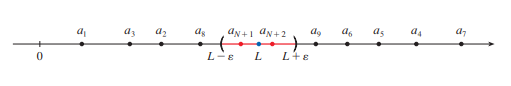
\includegraphics[width=0.6\textwidth]{graph67.png}
  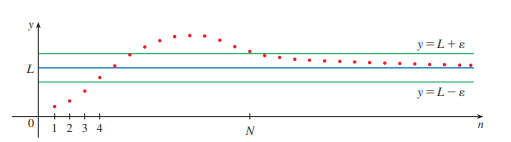
\includegraphics[width=0.6\textwidth]{graph68.png}
\end{figure}

\begin{tcolorbox}[colback=white, colframe=orange!80!white, title=Definition of a Limit of a Sequence (Precise), boxrule=0.5mm, arc=3mm]
A sequence \(\{a_n\}\) has the limit \(L\) if for every \( \varepsilon > 0 \), there is a corresponding integer \(N\) such that
\[ \text{if } n > N \quad \text{then} \quad |a_n - L| < \varepsilon \]
\end{tcolorbox}

\begin{tcolorbox}[colback=white, colframe=orange!80!white, title=Theorem 1, boxrule=0.5mm, arc=3mm]
If \( \lim_{x\to\infty} f(x) = L \) and \(f(n) = a_n\) when \(n\) is an integer, then \( \lim_{n\to\infty} a_n = L \).
\end{tcolorbox}

\begin{figure}[htbp]
  \centering
  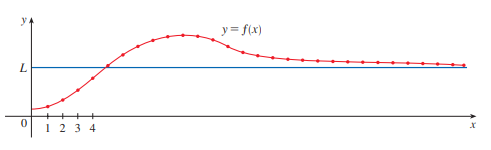
\includegraphics[width=0.5\textwidth]{graph69.png}
\end{figure}

\begin{tcolorbox}[colback=white, colframe=orange!80!white, title=Limit Laws for Sequences (Theorem 2), boxrule=0.5mm, arc=3mm]
If \(\{a_n\}\) and \(\{b_n\}\) are convergent sequences and \(c\) is a constant, then
\begin{itemize}
    \item[(a)] \( \lim_{n\to\infty} (a_n + b_n) = \lim_{n\to\infty} a_n + \lim_{n\to\infty} b_n \)
    \item[(b)] \( \lim_{n\to\infty} (a_n - b_n) = \lim_{n\to\infty} a_n - \lim_{n\to\infty} b_n \)
    \item[(c)] \( \lim_{n\to\infty} ca_n = c \lim_{n\to\infty} a_n \)
    \item[(d)] \( \lim_{n\to\infty} (a_n b_n) = (\lim_{n\to\infty} a_n) \cdot (\lim_{n\to\infty} b_n) \)
    \item[(e)] \( \lim_{n\to\infty} \dfrac{a_n}{b_n} = \dfrac{\lim_{n\to\infty} a_n}{\lim_{n\to\infty} b_n} \) if \( \lim_{n\to\infty} b_n \neq 0 \)
    \item[(f)] \( \lim_{n\to\infty} a_n^p = \left[\lim_{n\to\infty} a_n\right]^p \) if \(p>0\) and \(a_n>0\)
\end{itemize}
\end{tcolorbox}

\begin{tcolorbox}[colback=white, colframe=orange!80!white, title=The Squeeze Theorem for Sequences (Theorem 3), boxrule=0.5mm, arc=3mm]
If \(a_n \le b_n \le c_n\) for \(n \ge n_0\) and \( \lim_{n\to\infty} a_n = \lim_{n\to\infty} c_n = L \), then \( \lim_{n\to\infty} b_n = L \).
\end{tcolorbox}

\begin{figure}[htbp]
  \centering
  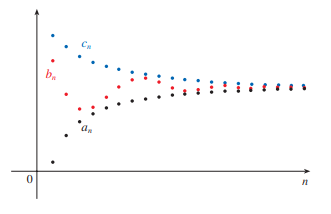
\includegraphics[width=0.4\textwidth]{graph70.png}
\end{figure}

\begin{tcolorbox}[colback=white, colframe=orange!80!white, title=Theorem 4, boxrule=0.5mm, arc=3mm]
If \( \lim_{n\to\infty} |a_n| = 0 \), then \( \lim_{n\to\infty} a_n = 0 \).
\end{tcolorbox}
\begin{proof}
Given \( \lim_{n\to\infty} |a_n| = 0 \). For any \(\varepsilon > 0\), there is an integer \(N\) such that if \(n>N\) then \(||a_n|-0| < \varepsilon\), which means \(|a_n| < \varepsilon\). But \( -|a_n| \le a_n \le |a_n| \). Since \(|a_n|<\varepsilon\), we have \(-\varepsilon < a_n < \varepsilon\), which implies \(|a_n - 0| < \varepsilon\). Therefore, \( \lim_{n\to\infty} a_n = 0 \).
\end{proof}

\subsection*{EXAMPLE 4 - 9: Calculating Limits}
\textbf{Ex 4:} Find \(\lim_{n\to\infty} \dfrac{n}{n+1}\).\\
 \textbf{SOLUTION:} Divide numerator and denominator by \(n\): \(\lim_{n\to\infty} \dfrac{1}{1+1/n} = 1\).\\\\
\textbf{Ex 5:} Find \(\lim_{n\to\infty} \dfrac{\ln n}{n}\).\\
 \textbf{SOLUTION:} Use L'Hospital's Rule on \(f(x) = \dfrac{\ln x}{x}\). \(\lim_{x\to\infty} \dfrac{1/x}{1} = 0\).\\
\textbf{Ex 6:} Does \(a_n = (-1)^n\) converge?\\
 \textbf{SOLUTION:} No, it oscillates between 1 and -1. Divergent.\\
\textbf{Ex 7:} Find \(\lim_{n\to\infty} \dfrac{(-1)^n}{n}\).\\
 \textbf{SOLUTION:} \(\lim_{n\to\infty} |\dfrac{(-1)^n}{n}| = \lim_{n\to\infty} \dfrac{1}{n} = 0\). By Thm 4, the limit is 0.\\
\textbf{Ex 8:} Discuss convergence of \(a_n = \dfrac{n!}{n^n}\).\\
 \textbf{SOLUTION:} Use Squeeze Theorem. \(0 < a_n = \dfrac{1 \cdot 2 \cdots n}{n \cdot n \cdots n} \le \dfrac{1}{n}\). Since \(\lim_{n\to\infty} \dfrac{1}{n} = 0\), the limit is 0.

 \begin{tcolorbox}[colback=white, colframe=orange!80!white, title=Theorem 4, boxrule=0.5mm, arc=3mm]
  If \( \lim_{n\to\infty} |a_n| = L \), then the function \(f\) is contivuous at \(L\), then \( \lim_{n\to\infty} f(a_n) = f(L) \).
\end{tcolorbox}

\textbf{Ex 9:} Evaluate \(\lim_{n\to\infty} \sin(\pi/n)\).\\
 \textbf{SOLUTION:} Since \(\sin x\) is continuous at 0, \(\lim_{n\to\infty} \sin(\pi/n) = \sin(\lim_{n\to\infty} \pi/n) = \sin(0) = 0\).

\subsection*{EXAMPLE 10}
 Discuss the convergence of the sequence \(a_n = \dfrac{n!}{n^n}\), where \(n! = 1 \cdot 2 \cdot 3 \cdots n\).\\
\textbf{SOLUTION:}
 Both the numerator and the denominator approach infinity as \(n \to \infty\).
 \[ a_1 = 1 \qquad a_2 = \frac{1 \cdot 2}{2 \cdot 2} \qquad a_3 = \frac{1 \cdot 2 \cdot 3}{3 \cdot 3 \cdot 3} \]
 \[ a_n = \frac{1 \cdot 2 \cdot 3 \cdots n}{n \cdot n \cdot n \cdots n} = \frac{1}{n} \left( \frac{2 \cdot 3 \cdots n}{n \cdot n \cdots n} \right) \]
 From this expression, it's clear that \(a_n\) is positive. We can also see that
 \[ 0 < a_n \le \frac{1}{n} \]
 because the fraction in the parentheses is less than or equal to 1. We know that \(\lim_{n\to\infty} 1/n = 0\). Therefore, by the Squeeze Theorem, we have
 \[ \lim_{n\to\infty} a_n = \lim_{n\to\infty} \frac{n!}{n^n} = 0 \]
 
\subsection*{EXAMPLE 11}
 For what values of \(r\) is the sequence \(\{r^n\}\) convergent?\\
\textbf{SOLUTION:}
 From the limits of exponential functions, we know that \(\lim_{x\to\infty} r^x = \infty\) for \(r>1\) and \(\lim_{x\to\infty} r^x = 0\) for \(0 < r < 1\). Therefore, putting \(a_n = r^n\), we have
 \[ \lim_{n\to\infty} r^n = \begin{cases} \infty & \text{if } r > 1 \\ 0 & \text{if } 0 < r < 1 \end{cases} \]
 For \(r=1\), \(\lim_{n\to\infty} 1^n = \lim_{n\to\infty} 1 = 1\).
 For \(r=0\), the sequence is \(\{0, 0, \dots\}\) and converges to 0.
 If \(-1 < r < 0\), then \(0 < |r| < 1\), so \(\lim_{n\to\infty} |r^n| = \lim_{n\to\infty} |r|^n = 0\), and \(\lim_{n\to\infty} r^n = 0\).
 If \(r \le -1\), the sequence \(\{r^n\}\) diverges.\\
 In summary, the sequence \(\{r^n\}\) is convergent if \(-1 < r \le 1\) and \[ \lim_{n\to\infty} r^n = \begin{cases} 0 & \text{if } -1 < r < 1 \\ 1 & \text{if } r = 1 \end{cases} \]

\section*{Monotonic and Bounded Sequences}
\begin{tcolorbox}[colback=white, colframe=orange!80!white, title=Definitions, boxrule=0.5mm, arc=3mm]
A sequence \(\{a_n\}\) is called \textbf{increasing} if \(a_n \le a_{n+1}\) for all \(n \ge 1\). \\
It is called \textbf{decreasing} if \(a_n \ge a_{n+1}\) for all \(n \ge 1\). \\
A sequence is \textbf{monotonic} if it is either increasing or decreasing.
\end{tcolorbox}

\subsection*{EXAMPLE 12}
Show that the sequence \(a_n = \dfrac{n}{n^2+1}\) is decreasing.\\
\textbf{SOLUTION:}
We must show that \(a_{n+1} \le a_n\), that is \(\dfrac{n+1}{(n+1)^2+1} \le \dfrac{n}{n^2+1}\).
This inequality is equivalent to \((n+1)(n^2+1) \le n((n+1)^2+1)\).
\begin{align*}
    n^3 + n + n^2 + 1 &\le n(n^2 + 2n + 1 + 1) \\
    n^3 + n^2 + n + 1 &\le n^3 + 2n^2 + 2n \\
    1 &\le n^2 + n
\end{align*}
Since \(n \ge 1\), this inequality is certainly true.

\subsection*{EXAMPLE 13}
Investigate the sequence defined by the recurrence relation \(a_1 = 2\), \(a_{n+1} = \dfrac{1}{2}(a_n+6)\) for \(n \ge 1\).\\
\textbf{SOLUTION:}
We begin by computing the first few terms:
\[ a_1 = 2 \quad a_2 = \frac{1}{2}(2+6) = 4 \quad a_3 = \frac{1}{2}(4+6) = 5 \quad a_4 = \frac{1}{2}(5+6) = 5.5 \]
These initial terms suggest that the sequence is increasing and the terms are approaching 6.\\
To confirm this, use mathematical induction to show that \(\{a_n\}\) is increasing and bounded above by 6.

\begin{tcolorbox}[colback=white, colframe=orange!80!white, title=Definitions, boxrule=0.5mm, arc=3mm]
A sequence \(\{a_n\}\) is \textbf{bounded above} if there is a number \(M\) such that \(a_n \le M\) for all \(n \ge 1\). \\
It is \textbf{bounded below} if there is a number \(m\) such that \(m \le a_n\) for all \(n \ge 1\). \\
If it is bounded above and below, then \(\{a_n\}\) is a \textbf{bounded sequence}.
\end{tcolorbox}

For instance, the sequence $a_n = n$ is bounded below ($a_n > 0$) but not above. The sequence $a_n = \dfrac{n}{n+1}$ is bounded because $0 < a_n < 1$ for all $n$.

We know that not every bounded sequence is convergent [for instance, the sequence $a_n = (-1)^n$ satisfies $-1 \le a_n \le 1$ but is divergent] and not every monotonic sequence is convergent ($a_n = n \to \infty$).\\
But if a sequence is both bounded and monotonic, then it must be convergent.
\begin{figure}[htbp]
  \centering
  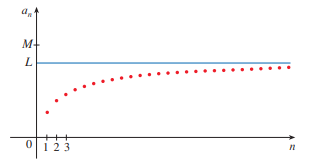
\includegraphics[width=0.35\textwidth]{graph71.png}
\end{figure}

\begin{tcolorbox}[colback=white, colframe=orange!80!white, title=Monotonic Sequence Theorem (Theorem 6), boxrule=0.5mm, arc=3mm]
Every bounded, monotonic sequence is convergent.
\end{tcolorbox}


\begin{proof}
Let \(\{a_n\}\) be an increasing sequence. Since \(\{a_n\}\) is bounded, the set \(S = \{a_n | n \ge 1\}\) has an upper bound. By the Completeness Axiom of the real numbers, \(S\) has a least upper bound \(L = \sup S\). We will show that \(\lim_{n\to\infty} a_n = L\).

Given \(\varepsilon > 0\), \(L-\varepsilon\) is not an upper bound for \(S\) (since \(L\) is the *least* upper bound). Therefore, there exists an integer \(N\) such that \(a_N > L - \varepsilon\).

Because the sequence is increasing, we have \(a_n \ge a_N\) for every \(n > N\). Thus, for \(n > N\), we have
\[ a_n > L - \varepsilon \]
Since \(L\) is an upper bound for \(S\), we also have \(a_n \le L\) for all \(n\). Therefore, for \(n > N\), we have
\[ L - \varepsilon < a_n \le L \]
This implies \(|a_n - L| < \varepsilon\) for all \(n > N\). Thus, by definition, \(\lim_{n\to\infty} a_n = L\).

A similar proof can be constructed for a decreasing sequence bounded below.
\end{proof}

\subsection*{EXAMPLE 14}
Investigate the sequence defined by \(a_1=2, a_{n+1}=\dfrac{1}{2}(a_n+6)\).\\
\textbf{SOLUTION:} By induction, one can show the sequence is increasing and bounded above by 6, so it converges. Let \(L = \lim_{n\to\infty} a_n\). Then \(L = \dfrac{1}{2}(L+6)\), which gives \(2L=L+6\), so \(L=6\).\\
\textbf{Boundedness:} We show that \(a_n < 6\) for all \(n \ge 1\).
This is true for \(n=1\) since \(a_1 = 2 < 6\). Assume that \(a_k < 6\) for some \(k \ge 1\). Then
\[ a_{k+1} = \dfrac{1}{2}(a_k+6) < \dfrac{1}{2}(6+6) = 6 \]
Thus \(a_{n+1} < 6\) whenever \(a_n < 6\). So the sequence is bounded above by 6. It is also bounded below by 2 since \(a_n\) is increasing.\\
\textbf{Monotonicity:} We show that \(a_{n+1} \ge a_n\) for all \(n \ge 1\).
\[ a_2 - a_1 = 4-2=2 > 0 \]
Assume that \(a_{k+1} > a_k\) for some \(k \ge 1\). Then \(a_k < a_{k+1}\), so \(a_k+6 < a_{k+1}+6\), and \(\dfrac{1}{2}(a_k+6) < \dfrac{1}{2}(a_{k+1}+6)\). Thus \(a_{k+1} < a_{k+2}\). By the principle of mathematical induction, \(a_{n+1} \ge a_n\) for all \(n\).
Since the sequence \(\{a_n\}\) is bounded and increasing, it is convergent by the Monotonic Sequence Theorem. The limit must be 6.

\end{document}